\setcounter{section}{99}
\section{Доказательство теоремы Минковского-Главки для октаэдра: переформулировка условия теоремы через $\Lambda_a$ и неравенства на p и n. Сведение теоремы к неравенству}
\textbf{Теорема Минковского-Главки}: $\frac{Vol \Omega}{\Delta(\Omega)} \geqslant 1$, где $\Omega$ - произвольное тело; мы работаем с ней для октаэдра, но не на классе ВСЕХ решёток (в критическом определителе у нас inf по всем решёткам), а переформулируем: \\
$\forall \varepsilon > 0 \exists n_0 \forall n \geqslant n_0 \exists \Lambda \subset \mathbb{R}^n: \Lambda \cap \Omega \backslash \{0\} = \varnothing$, а $\det \Lambda \leqslant (Vol \Omega)(1 + \varepsilon)$ \\
Рассмотрим $\overline{a} = (a_1/p, a_2/p, \dots, a_n/p)$, p - простое число, $a_i \in \mathbb{Z}$. Берём $<\mathbb{Z}^n, \overline{a}>$ = $\{\overline{a}l + \overline{b}: l \in \mathbb{Z}, \overline{b} \in \mathbb{Z}^n\}$. Тогда $\Lambda_{\overline{a}}$ = $<\mathbb{Z}^n, \overline{a}>$- это вот эта решётка. Б.о.о. $1 \leqslant a_i \leqslant p - 1$. \par
\textbf{Утверждение}: $\det\Lambda_{\overline{a}} = \frac{1}{p}$ \par
$\textbf{Переформулировка условия теоремы Минковского-Главки}$ $\forall \varepsilon > 0 \exists n_0 \forall n \geqslant n_0 \exists \Lambda_{\overline{a}} \subset \mathbb{R}^n: \Lambda_{\overline{a}} \cap O^n \backslash \{0\} = \varnothing$ ($\Lambda_{\overline{a}}$ допустима относительно $O^n$, а $\det \Lambda_{\overline{a}} = \frac{1}{p} \leqslant (Vol O^n)(1 + \varepsilon) = \frac{2^n}{n!}(1+\varepsilon)$, что, по сути, $p \geqslant \frac{n!}{2^n}(1-\varepsilon)$ \\
\\
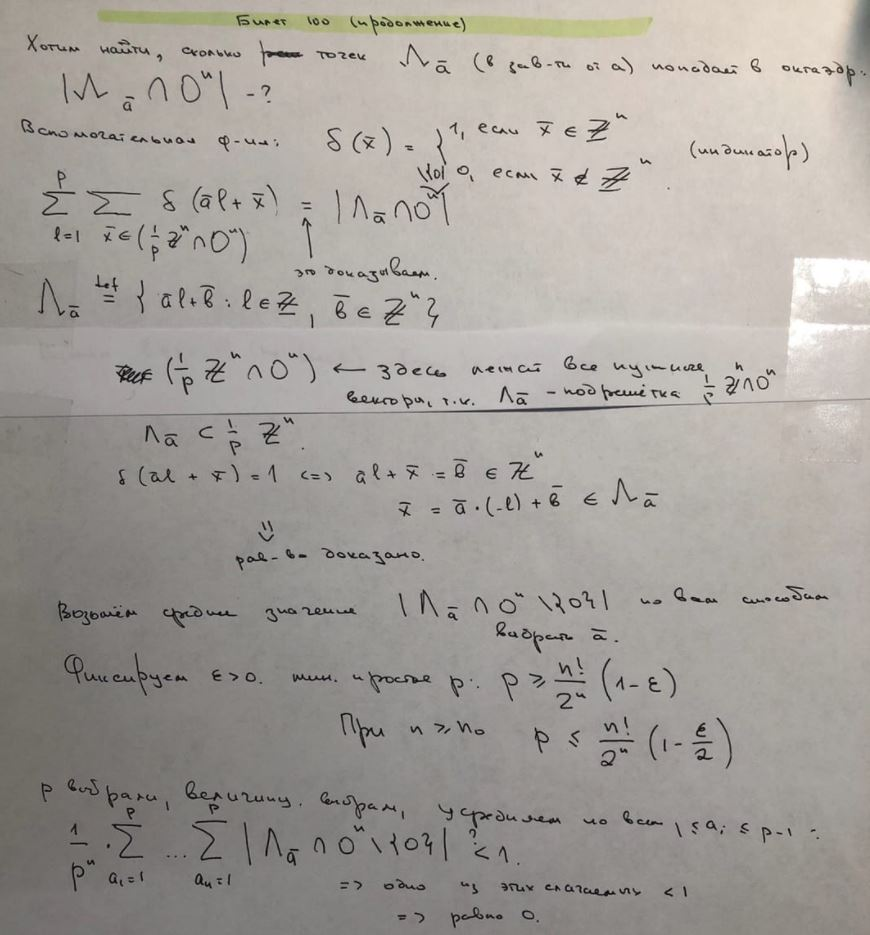
\includegraphics[width=15cm]{images/100_1}

\section{Теорема Минковского-Главки для октаэдра (формулировка). Доказательство неравенства.}
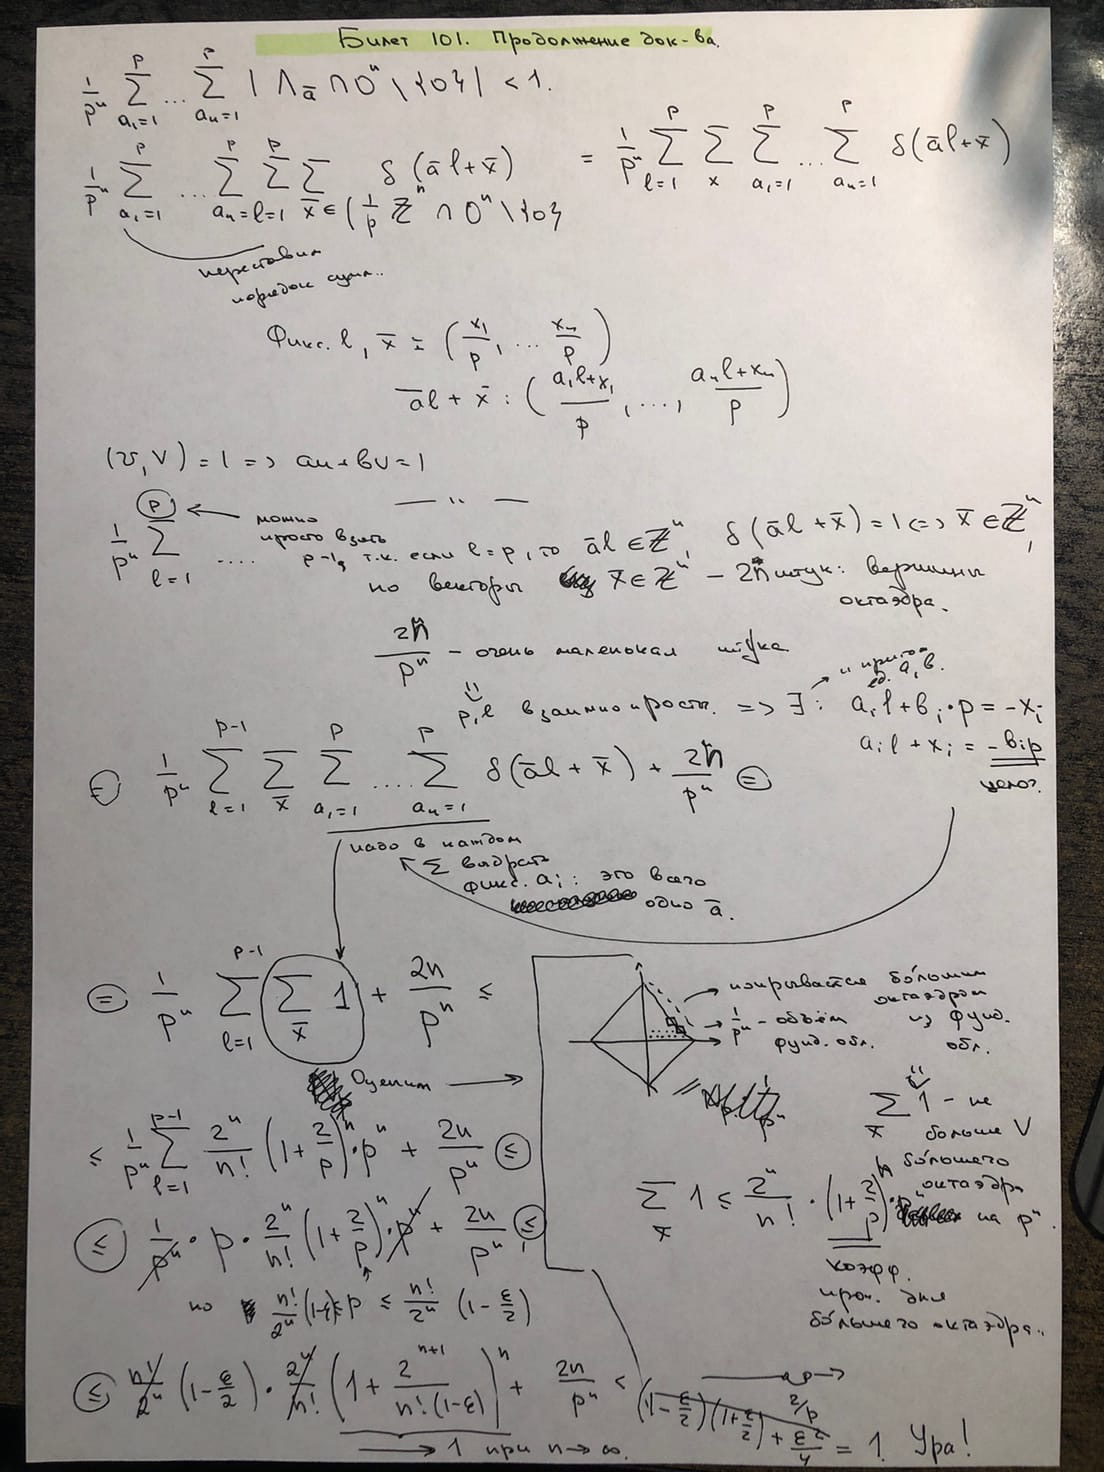
\includegraphics[width=15cm]{images/100_2}